

\newpage

\begin{center}
{\includegraphics[scale=1]{om.eps}}\\[5pt]

{\normalsize ಶ್ರೀ ಸದ್ಗುರವೇ ನಮಃ }\\[5pt]

{\large ಅಷ್ಟಾಂಗಯೋಗವಿಜ್ಞಾನಮಂದಿರಂ}
\end{center}

\vskip -20pt

\begin{figure}[h]
\centerline
{
\includegraphics[scale=.18]{0000d.eps}}
\end{figure}

ಸತ್ಯಜ್ಞಾನಾನಂತಸ್ಯ, ಶ್ರೀಭಾರತೀಭರತಾಚಾರ್ಯಸ್ಯ, ವಿದ್ಯಾರಾಜಸ್ಯ, ಜ್ಞಾನ ಯಜ್ಞಮುದ್ರಾನ್ವಿತಸ್ಯ, ಹಂಸವಿಜ್ಞಾನೋಪದೇಷ್ಟು, ಅಮೃತರಸಧಾರಾವರ್ಷಿಣಃ ವಿಶ್ವಭಾರತಶ್ರೇಯಃಪ್ರೇಯವಿತರನವಿಶಾರದಸ್ಯ, ಪ್ರಣವಹಯಹಮ್ಸಪರೋರಜಸಃ, ಭಗವತೋ ಜ್ಯೋತಿರ್ನಾರಾಯಣಸ್ಯ ದಿವ್ಯಪದಯುಗಲೇ ಪ್ರಾಣಾನ್ ಪ್ರಣಾಮಯಾಮಃ|

ತ್ರಿವಿಕ್ರಮವಿಷ್ಣುಲಕ್ಷ್ಮೀನಿಕೇತನೇ, ಜ್ಞಾನವಿಜ್ಞಾನಮಂದಿರವ್ಯೋಮಾಂಬುಜೇ, ಮಹರ್ಷಿಹೃದಂತರ್ಲಕ್ಪ್ಯಸರ್ವವಿದ್ಯಾಮೂಲ ಜ್ಯೋತಿಃ  ಸಮೀಕ್ಷ್ಯ, ಭಾರತಭರತಾಃ ಆನಂದಭರಿತಾಃ ಮಯಮಸ್ಮಚ್ಚತುಷ್ಪಷ್ಟಿವಿದ್ಯಾಂತರ್ನಿಹಿತನ ತೇನ ಜ್ಞಾನವಿಜ್ಞಾನ ಮಯಮಹಾಹಯಹಂಸಜ್ಯೋತಿಸ್ಸ್ತಂಭಮೂಲದೀಪೇನ, ವಿಶ್ವವಿಜ್ಞಾನಮಂದಿರೇ ದೀಪಮಾಲಾಸಹಸ್ರಮುದ್ದೀಪಯಾಮ|

ಮಹಾಮಸ್ತಿಷ್ಕಜ್ಞಾನವಿಜ್ಞಾನವಿಜ್ಞಾನಮಂದಿರೇ ತ್ರಿಧಾಮಬ್ರಹ್ಮಮಾರ್ಗತತ್ತ್ವ  ಸೋಪಾನವಿಶ್ವರಂಗಾಂಬುಜೇ, ಹಂಸಾಸನಾಯಾಃ, ಹಂಸಗಮನಾಯಾಃ ನಾದಶಬ್ದಬ್ರಹ್ಮ ರೂಪಿಣ್ಯಾಃ ಬ್ರಹ್ಮದಂಡನೀತಿವಿವೃಣ್ವತ್ತ್ರಿಕಾಲಮೂರ್ತಿಸುಂದರ್ಯಾಃ ಜೀವನಸುಮನೋವಿಕಾಸಪ್ರಾಣಶಕ್ತ್ಯಾಃ, ಬ್ರಹ್ಮಭಾವಜ್ಯೋತಿರ್ನಾದವಿಜ್ಞಾನವಿಪಂಚಿಕಾಂ ಪ್ರಪಂಚ್ಯಾತ್ಮಶ್ರಿಯಮ್ ವ್ಯಾತನ್ವಾನಾಯಾಃ ವಿಶ್ವಶಿಲ್ಪವಿಧಾನಜ್ಞಾಯಾಃ, ಅಸ್ಮನ್ಮಂದಿರಮಹಾಮಂಗಲದೀಪರೇಖಾಯಾಃ , ವಿದ್ಯಾಧಿರಾಜ್ಞ್ಯಾಃ ಮಹಾನಾಟ್ಯಭಾರತ್ಯಾಃ, ದಿವ್ಯಪದಪುಂಡರೀಕಮಹಾಮಧು ನಿರಂತರಂ, ಅಸ್ಮತ್ಪ್ರಾಣಮಧುಕರಃ ಪೂರ್ಣಚಂದ್ರಿಕಾಯಾಂ ಆಸ್ವದಯತುತರಾಮ್ |||

\vskip 30pt

\centerline{\bf ಓಮ್ ತತ್ ಸತ್}


